% Downloaded MB
\begin{figure*}[t]
    \centering
    \subfloat[\textbf{Pre-lockdown weekdays.} Average volume of downloaded data per user, broken down by the hour of the day, on weekdays in the pre-lockdown time period. \label{download-a}]{%
       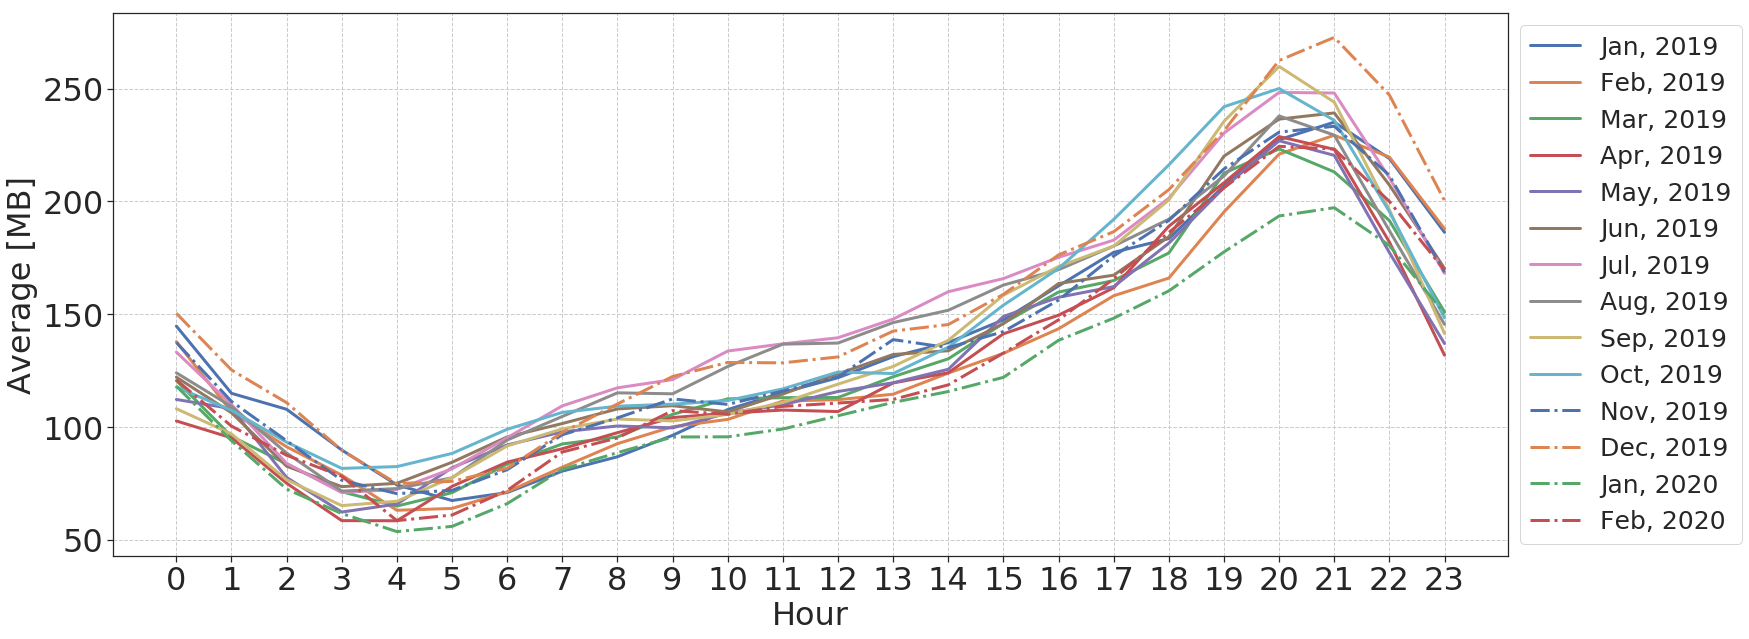
\includegraphics[width=0.48\linewidth]{figs/wenjun/download_wdays_before.png}%
    }
    \hspace{0.2cm}
    \subfloat[\textbf{Pre-lockdown weekends.} Average volume of downloaded data per user, broken down by the hour of the day, on weekends in the pre-lockdown time period. \label{download-b}]{%
        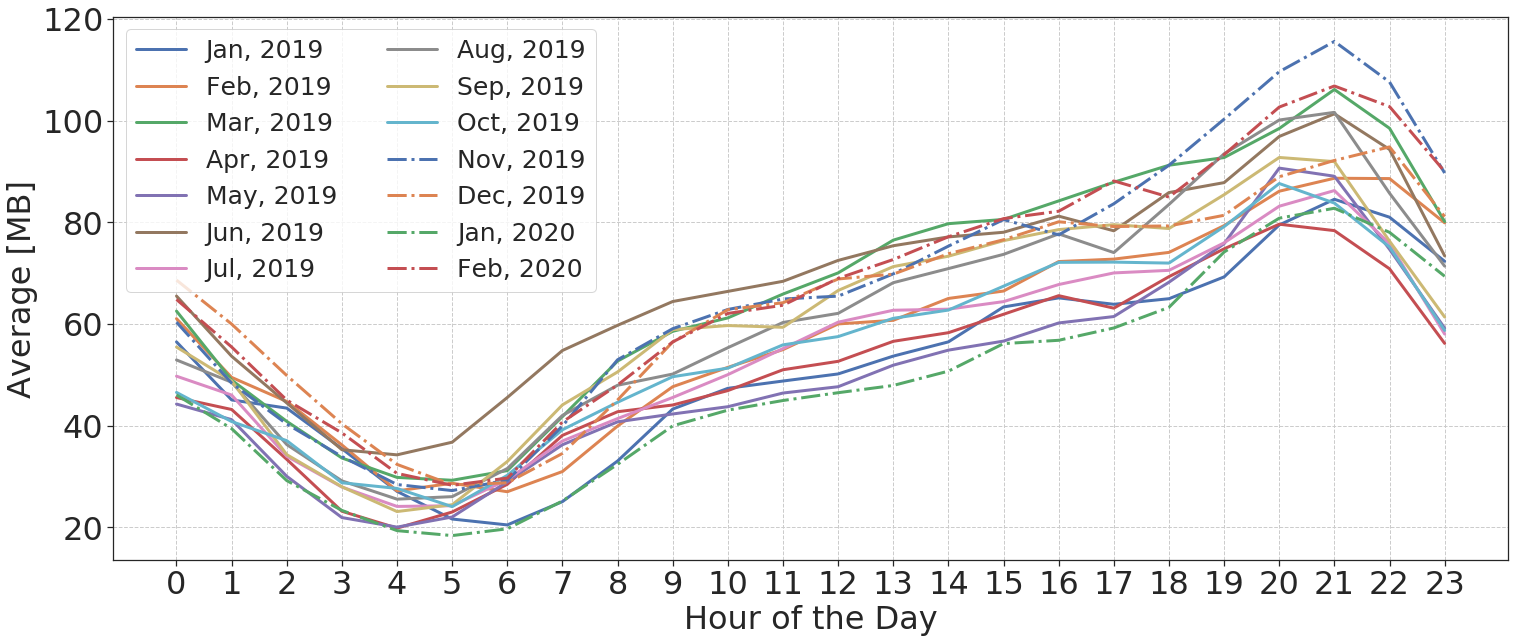
\includegraphics[width=0.48\linewidth]{figs/wenjun/download_wends_before.png}%
    }
    \\
    \subfloat[\textbf{Lockdown weekdays.} Average volume of downloaded data per user, broken down by the hour of the day, on weekdays in the lockdown time period. \label{download-c}]{%
        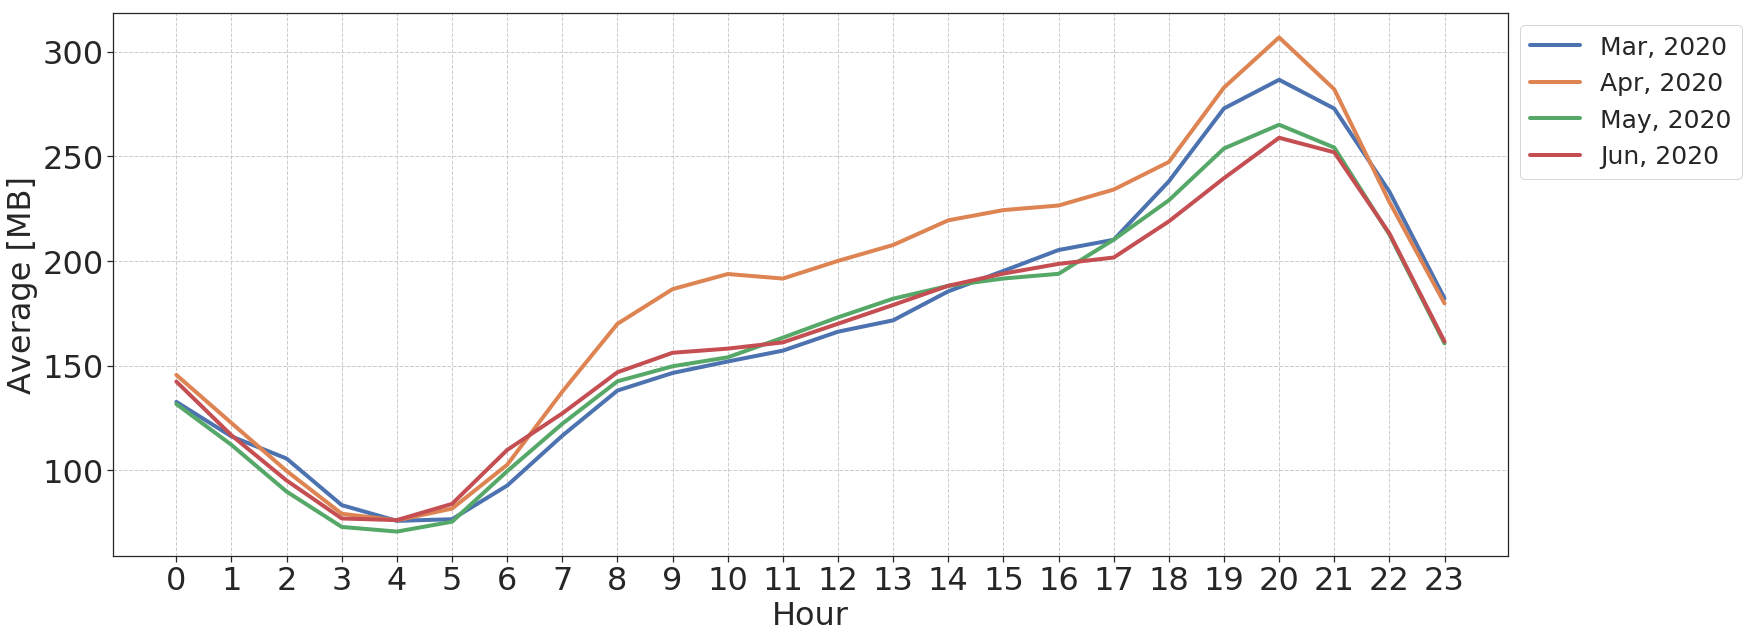
\includegraphics[width=0.48\linewidth]{figs/wenjun/download_wdays_after.png}%
    }
    \hspace{0.2cm}
    \subfloat[\textbf{Lockdown weekends.} Average volume of downloaded data per user, broken down by the hour of the day, on weekends in the lockdown time period. \label{download-d}]{%
        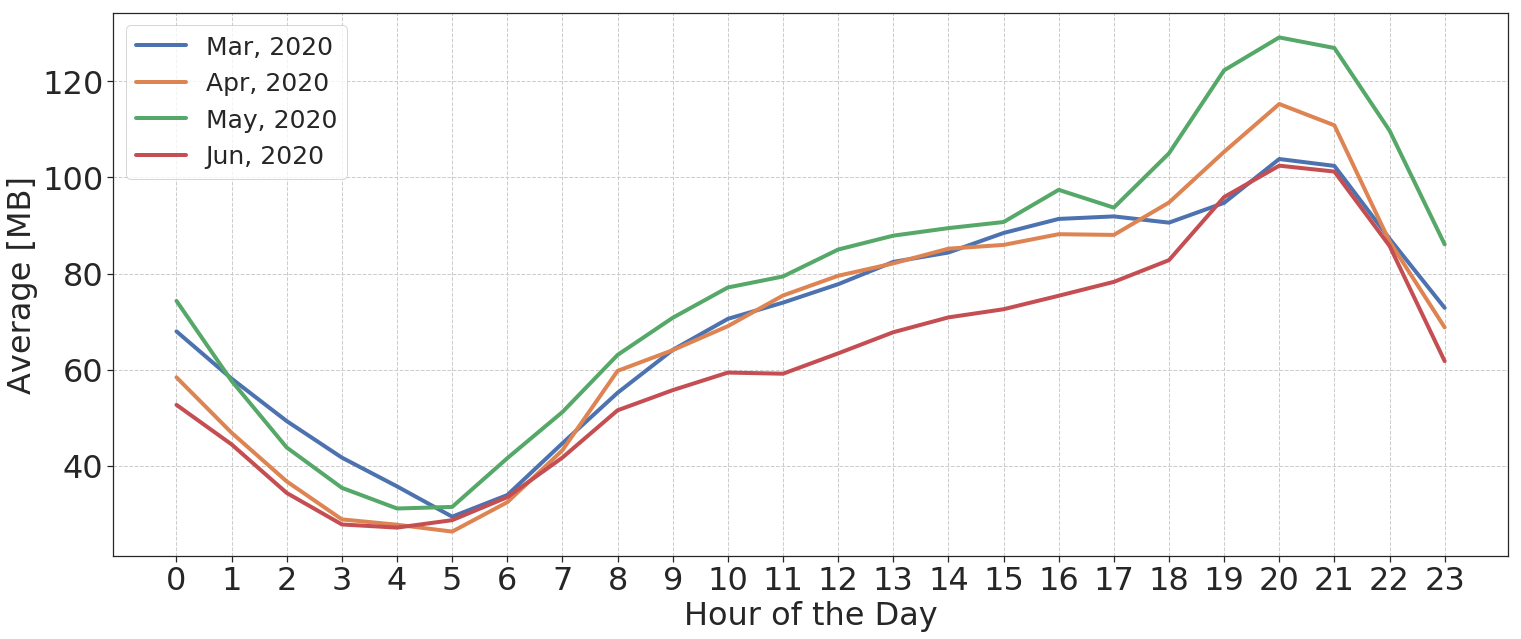
\includegraphics[width=0.48\linewidth]{figs/wenjun/download_wends_after.png}%
    }
    \\
    \subfloat[\textbf{2019 vs 2020 weekdays.} Average volume of downloaded data per user on weekdays in March-June compared between 2019 and 2020.
    \label{download-e}]{%
        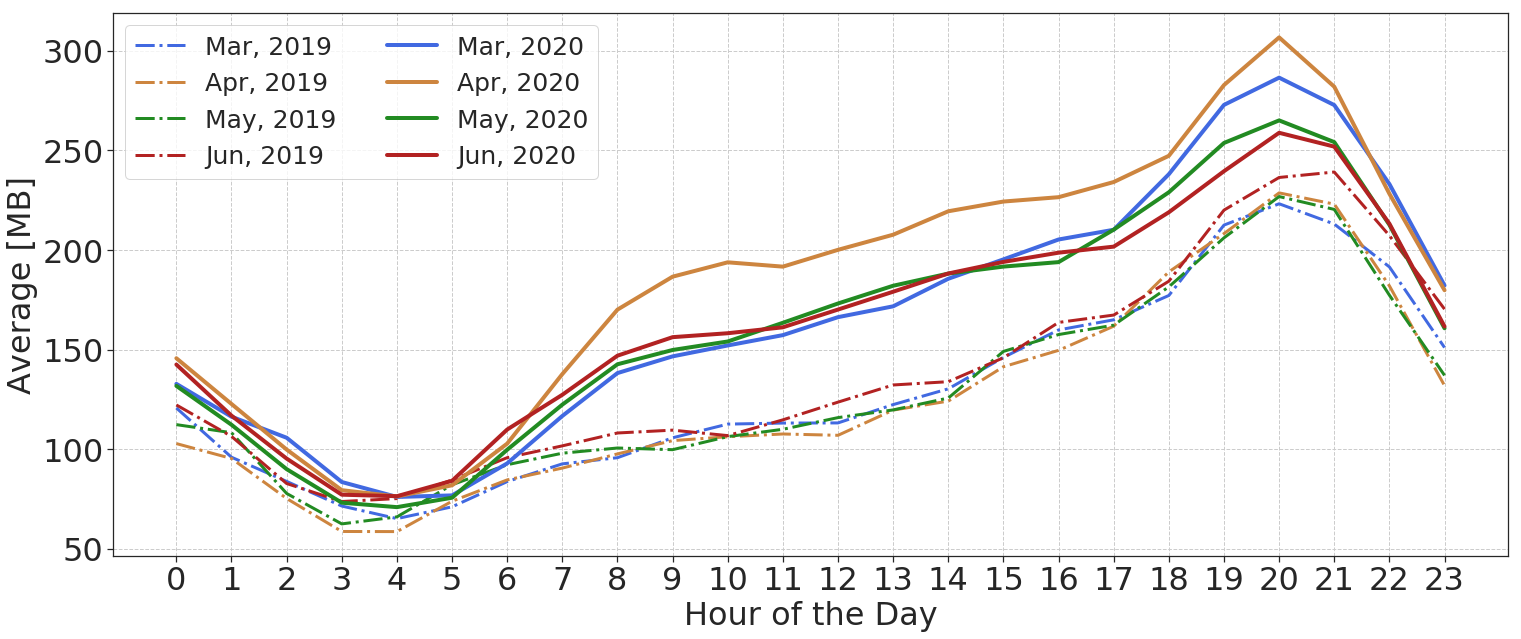
\includegraphics[width=0.48\linewidth]{figs/wenjun/download_wdays_compare_36.png}%
    }
    \hspace{0.2cm}
    \subfloat[\textbf{2019 vs 2020 weekends.} Average volume of downloaded data per user on weekends in March-June compared between 2019 and 2020.
    \label{download-f}]{%
        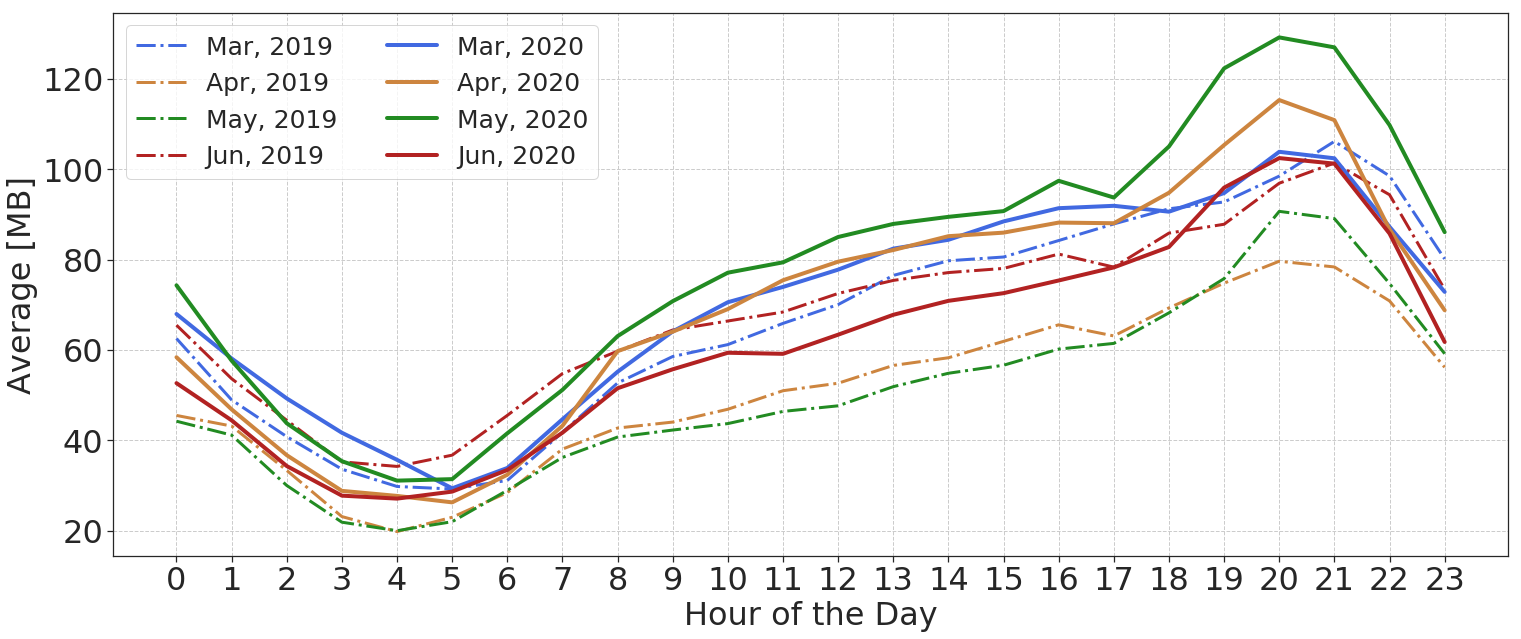
\includegraphics[width=0.48\linewidth]{figs/wenjun/download_wends_compare_36.png}%
    }
        
    \caption{Graphs comparing and contrasting the average hourly downloaded volume of data per user in various time periods. The peak is always between 18:00 and 22:00, which is the internet rush hour. The volumes in the lockdown time period are generally larger than the volumes in the pre-lockdown time period. Lockdown weekday traffic patterns start to resemble weekend patterns.
    }
    \label{fig:download-data-per-user-hours-fig}
\end{figure*}

\begin{figure*}[t]
    \centering
    \subfloat[Average Hourly Uploaded MB per User before COVID-19 on Weekdays
    \label{upload-a}]{%
        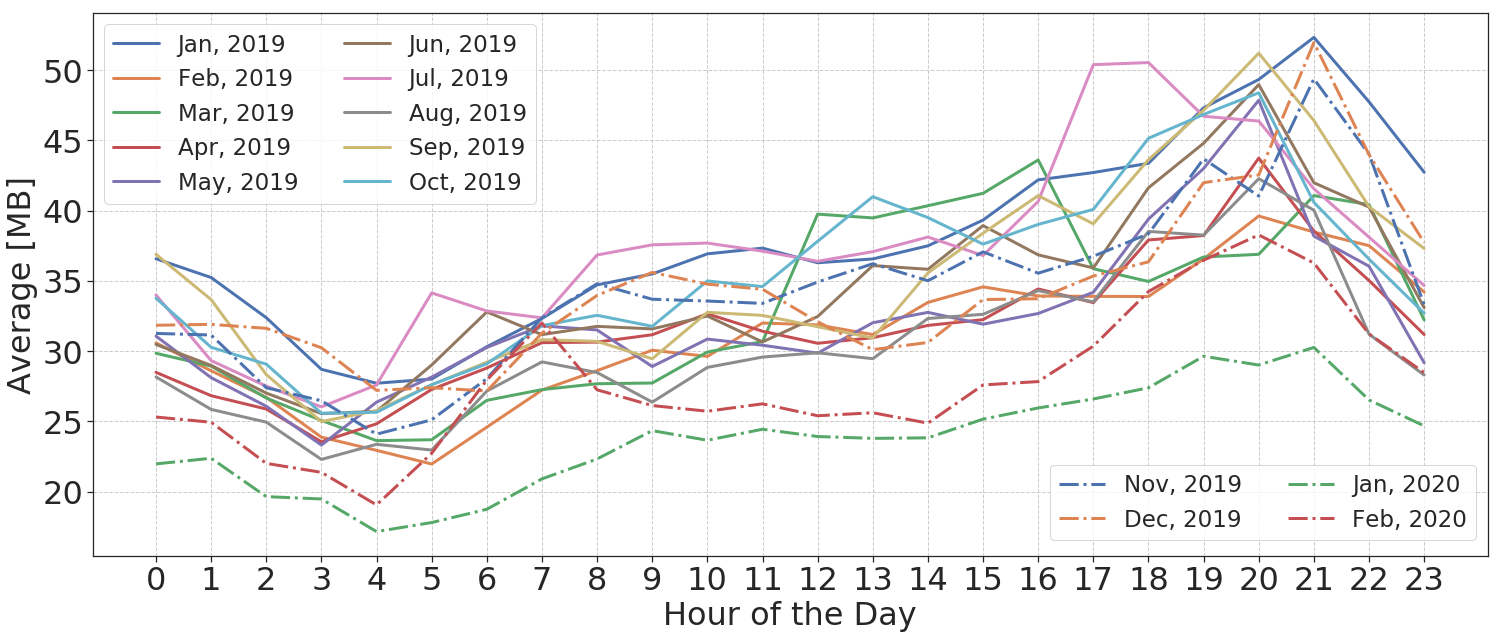
\includegraphics[width=0.48\linewidth]{figs/wenjun/upload_wdays_before.png}%
    }
    \hspace{0.2cm}
    \subfloat[Average Hourly Uploaded MB per User before COVID-19 on Weekends
    \label{upload-b}]{%
        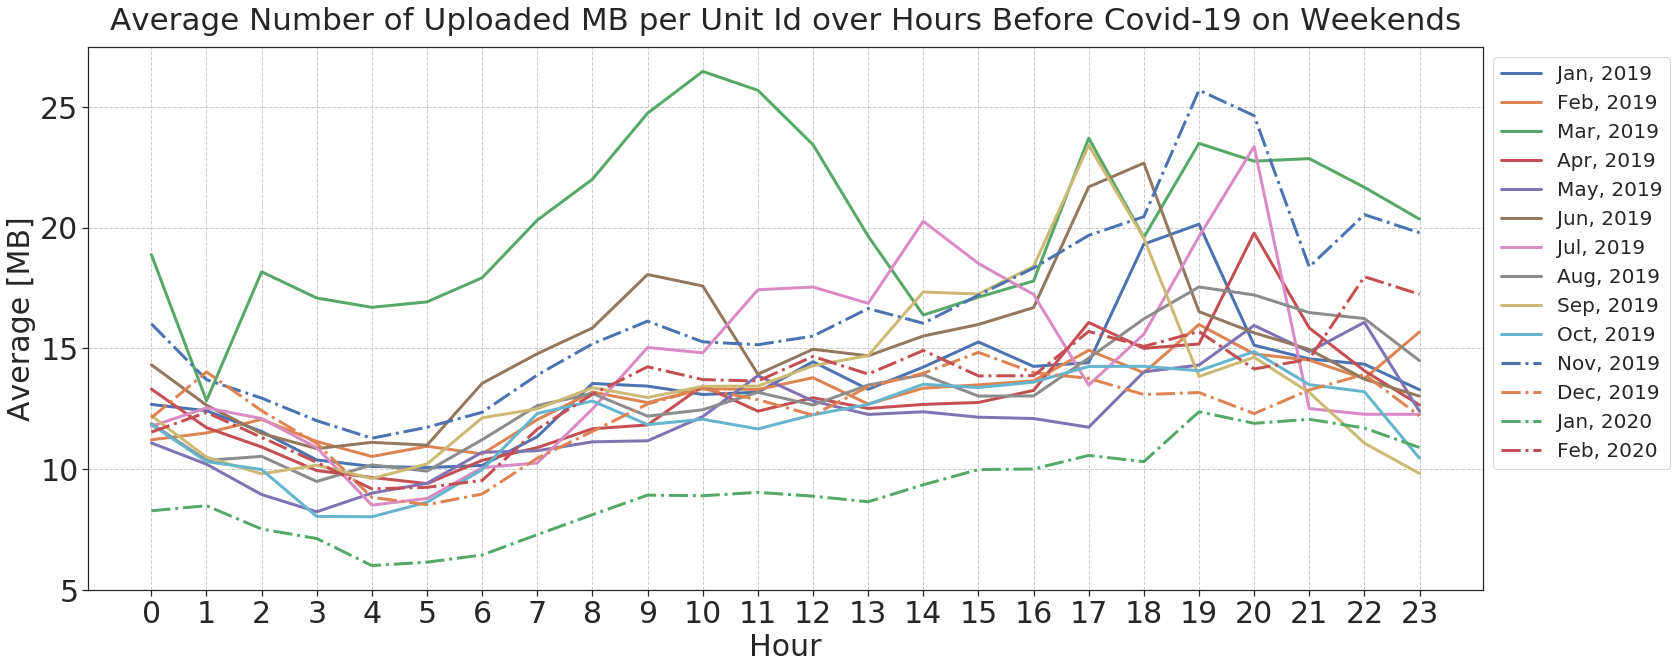
\includegraphics[width=0.48\linewidth]{figs/wenjun/upload_wends_before.png}%
    }
    \\
    \subfloat[Average Hourly Uploaded MB per User after COVID-19 on Weekdays
    \label{upload-c}]{%
        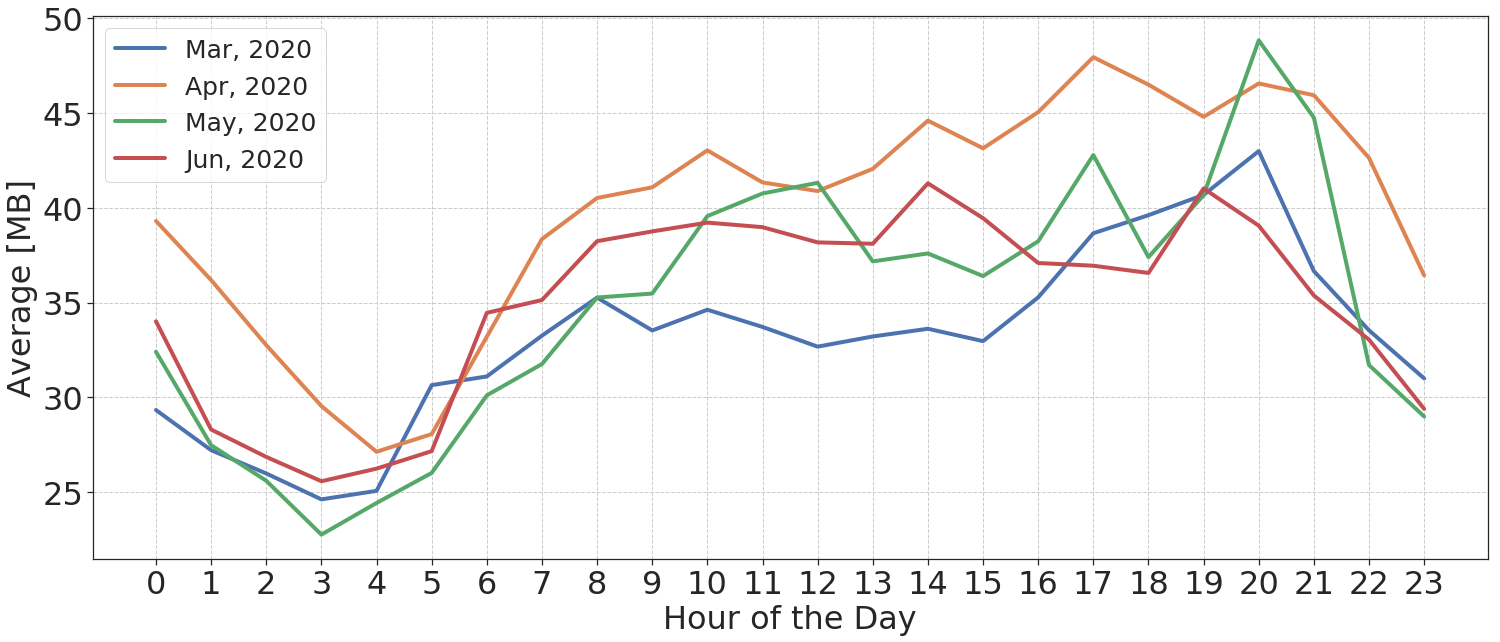
\includegraphics[width=0.48\linewidth]{figs/wenjun/upload_wdays_after.png}%
    }
    \hspace{0.2cm}
    \subfloat[Average Hourly Uploaded MB per User after COVID-19 on Weekends \label{upload-d}]{%
        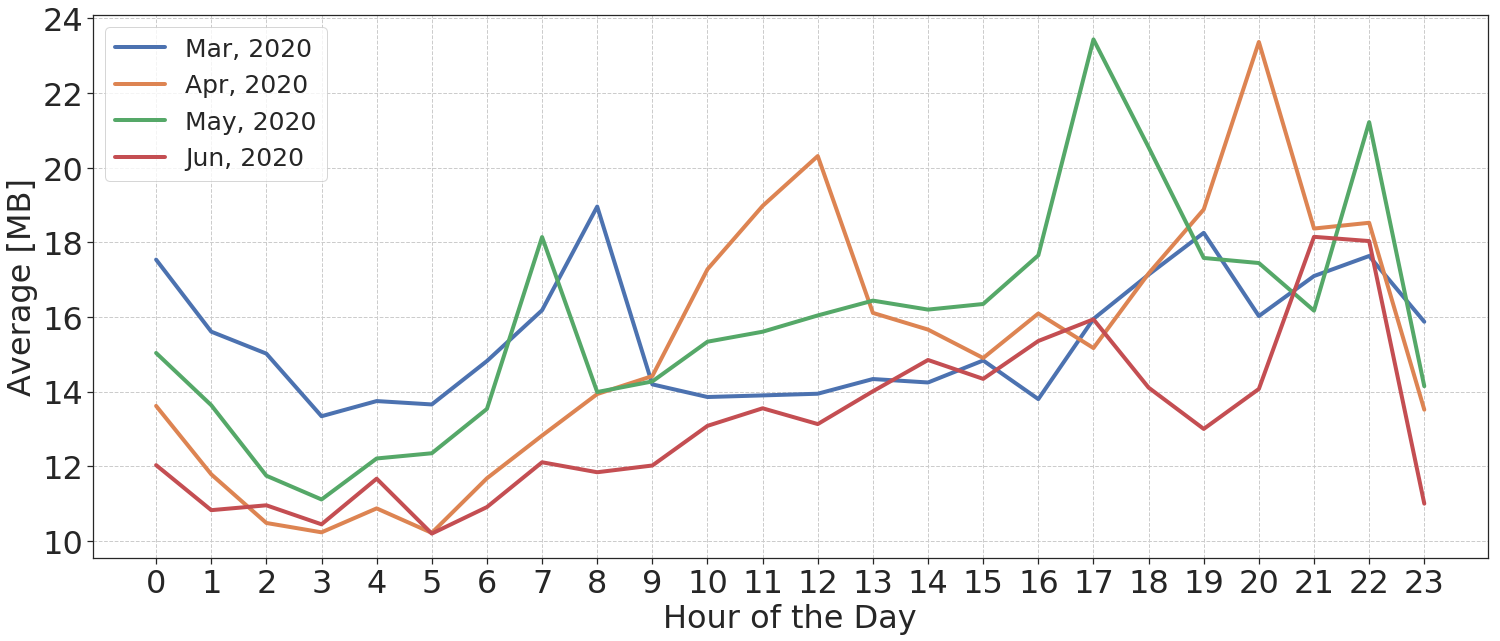
\includegraphics[width=0.48\linewidth]{figs/wenjun/upload_wends_after.png}%
    }
    \\
    \subfloat[March to June: Average Hourly Uploaded MB per User on Weekdays
    \label{upload-e}]{%
        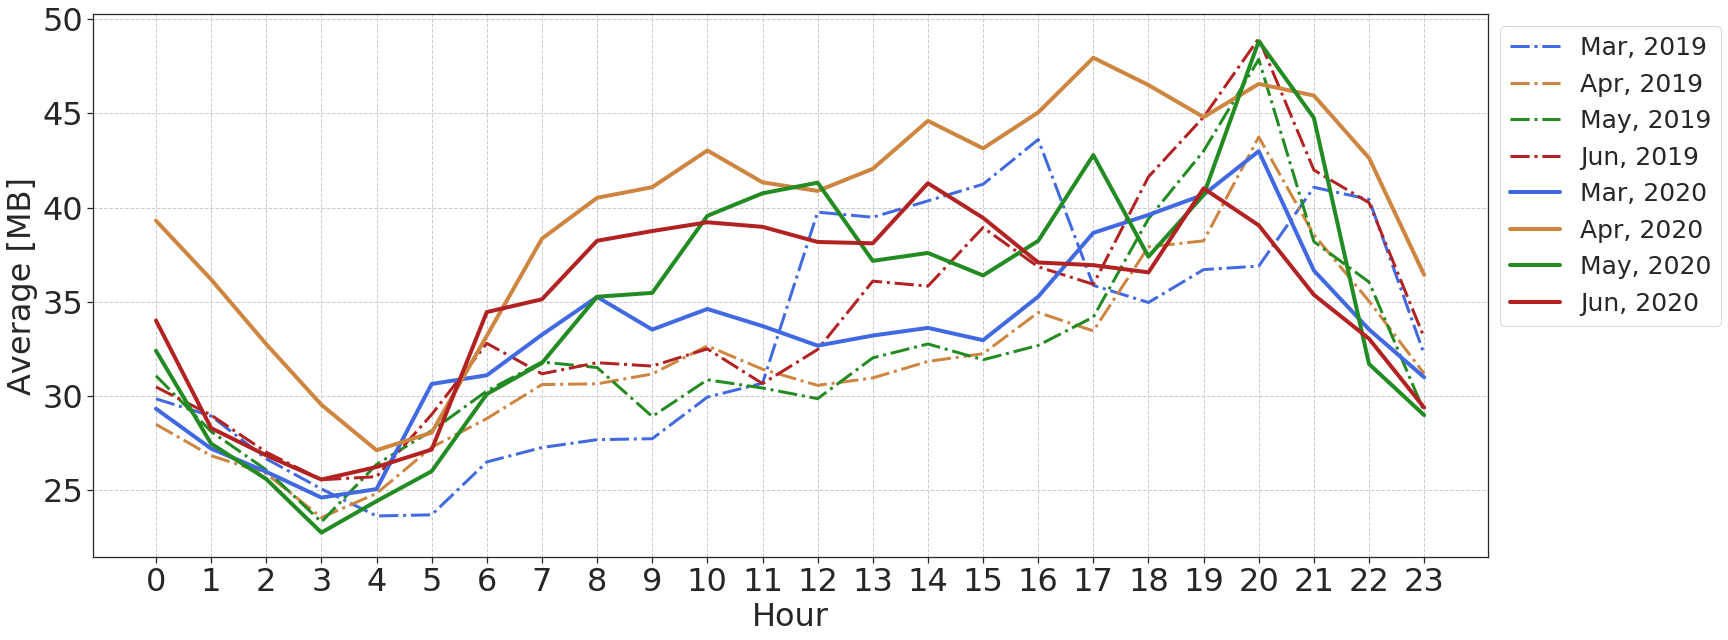
\includegraphics[width=0.48\linewidth]{figs/wenjun/upload_wdays_compare_36.png}%
    }
    \hspace{0.2cm}
    \subfloat[March to June: Average Hourly Uploaded MB per User on Weekends
    \label{upload-f}]{%
        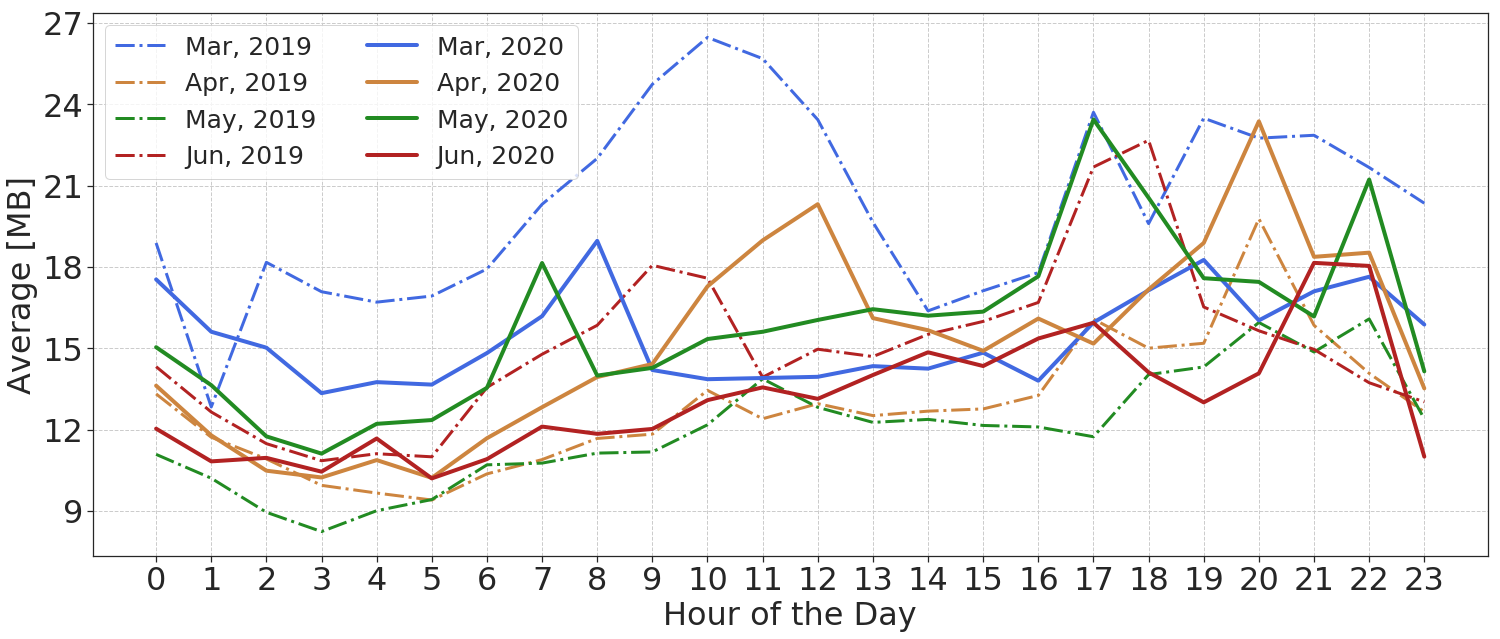
\includegraphics[width=0.48\linewidth]{figs/wenjun/upload_wends_compare_36.png}%
    }
        
    \caption{Graphs related to average hourly uploaded data per user in each month.           Compare with the pattern for average hourly downloaded data, the lines in the         uploaded data graph are more fluctuating, especially the pattern for the uploaded     data on weekends. In April and May, the average hourly uploaded data per user in      2020 is larger than those in 2019.
    }
  \label{fig:upload_data_per_user_hours_fig} 
\end{figure*}


\section{Daily Data Usage Patterns}

% \subsection{Hourly Data Usage Patterns}
Data will be consumed whenever people use internet, such as sending or receiving emails, downloading or uploading information (e.g., music, video), playing games, and so forth.
Through the data usage, we are able to know about how many internet people use for their daily activities during a certain period. As the average hourly data usage can reflect dialy patterns of users’ internet use behaviors, we study the average hourly data usage per user by month. In order to figure out how the internet use behaviors may be changed because of COVID-19, we additionally analyze differences between downloaded and uploaded data based on both weekdays and weekends, before and after the COVID-19 pandemic.

\subsection{Average Downloaded Data per User}
\label{sec:download-data-per-user-over-hours}

% The download data is the number of bytes that the customer received from the internet to wired LAN devices and the Wi-Fi devices. 

As shown in the Figure \ref{fig:download-data-per-user-hours-fig}, we can find that the patterns of downloaded data usage are the same on weekdays and weekends whether before COVID-19 or after COVID-19. There is a peak between 18:00 and 22:00, which is the internet rush hour \cite{internetrushhour}. A likely explanation for this peak is post-workday internet consumption in the form of Youtube, Netflix, etc. 

According to the Figure \ref{download-e} and Figure \ref{download-f}, the average downloaded data per user over hour after COVID-19 is larger than those before COVID-19. 

On weekdays (Figure \ref{download-e}), the gaps between average downloaded data per user from March to June in 2020 and average downloaded data per user in 2019 from 7:00 to 22:00 are more obvious than those from 22:00 to 7:00 next day. For the increase from 7:00 to 18:00, the possible reasons are work from home and online learning. Since the work-from-home period mainly takes place from April and May \cite{remotework}, the average hourly downloaded data per user in April increases the most in 2020. The increase from 18:00 to 22:00 is likely due to gathering and social contact restriction, and then people are not allowed to hang out with friends and dine in at the restaurant after work \cite{lockdownsguide}. Instead, people are supposed to stay at home. Watching streaming video or other recreational activities that require internet may be the first choice for most of the people, and these online activities will consume a lot of downloaded data. 22:00 to 7:00 the next day are generally reserved for sleep, so the lack of difference between downloaded data usage in these hours before and after COVID-19 is unsurprising. 

On weekends (Figure \ref{download-f}), there is a small rise for the average hourly downloaded data per user in March, and the increases in April and May are substantial. In June, the average hourly downloaded data per user in 2020 is not always larger than those in 2019. This pattern coincides with the policies related to COVID-19 in the United States: the height of restriction is at the end of March and the beginning of April, and some restrictions such as stay-at-home order are ended in the mid-late of May or in June at most of the states \cite{covid19restriction}. It 
implies that in April and May, people might need to stay at home and use internet the most. Since the restriction started in the middle of March, the average hourly downloaded data per user was not affected too much, and in June, some of the restrictions end and people may be able to reschedule the outdoor activities. Therefore, we may be able to conclude that people use more internet and download more data because of COVID-19 and its related policies (e.g., lockdown, quarantine, work from home, etc.). 

\subsection{Average Uploaded Data per User}
\label{sec:upload-data-per-user-over-hours}

% The upload data is the number of bytes that the customer transmitted from wired LAN devices and Wi-Fi devices to the internet. 

As evidenced in Figure \ref{fig:upload_data_per_user_hours_fig}, compare with the pattern in average hourly downloaded data, the lines in the uploaded data graph are more fluctuating, especially the pattern for the uploaded data on weekends.

Similar to average hourly downloaded data per user, we compare the average hourly uploaded data from March to June in 2020, the period after COVID-19, with those from March to June in 2019. It is shown that the average hourly uploaded data per user in April and May 2020 is larger than that in 2019, but in March and June, that is not the case (Figure \ref{upload-e} and \ref{upload-f}). The reasons might be similar to those of downloaded data: the peak of shelter-in-place and stay-at-home are 
at the end of March and the beginning of April, and the restrictions are ended in the mid-late of May or in June at some states \cite{covid19restriction}. On weekdays, potentially because of the policies such as work-from-home, the average upload data per user at daytime in April, May, and June 2020 are observed much larger than those in April, May, and June 2019. On weekends, the increase of uploaded data is relatively smaller than that on weekdays. One possible reason could be that weekend is a time to have a rest.  